\section{Methods}
% There are many methods for solving the object detection problem. 
% One way is using region proposal and region-based convolutional neural networks to make classification on different region proposals, such as R-CNN, Fast R-CNN, SPPnet, and Faster R-CNN, etc. Another way is 

\subsection{You Only Look Once (yolo)}
Yolo is a real-time object recognition algorithm. Unlike sliding window and region proposal-based techniques, it trains on full images and reframes object detection as a single regression problem.The yolo system firstly resizes images to 448*448, then runs a single convolutional network, and predicts multiple bounding boxes and class probabilities for those boxes. It only looks at images once, unlike R-CNN which require thousands for a single image. This makes yolo extremely fast, more than 1000x faster than R-CNN and 100x faster than Fast R-CNN. 

Yolo system divides an image into S × S grid. Each grid cell predicts B bounding boxes and C conditional class probabilities. Each bounding box contains 5 predictions: x, y, w, h, and confidence score. So the final prediction is a S × S × (B * 5 + C) sensor.

Yolo network has 24 convolutional layers followed by 2 fully connected layers.The initial convolutional layers extract features from the image while the fully connected layers predict the output probabilities and coordinates. 
\begin{figure}[H]
    \centering
    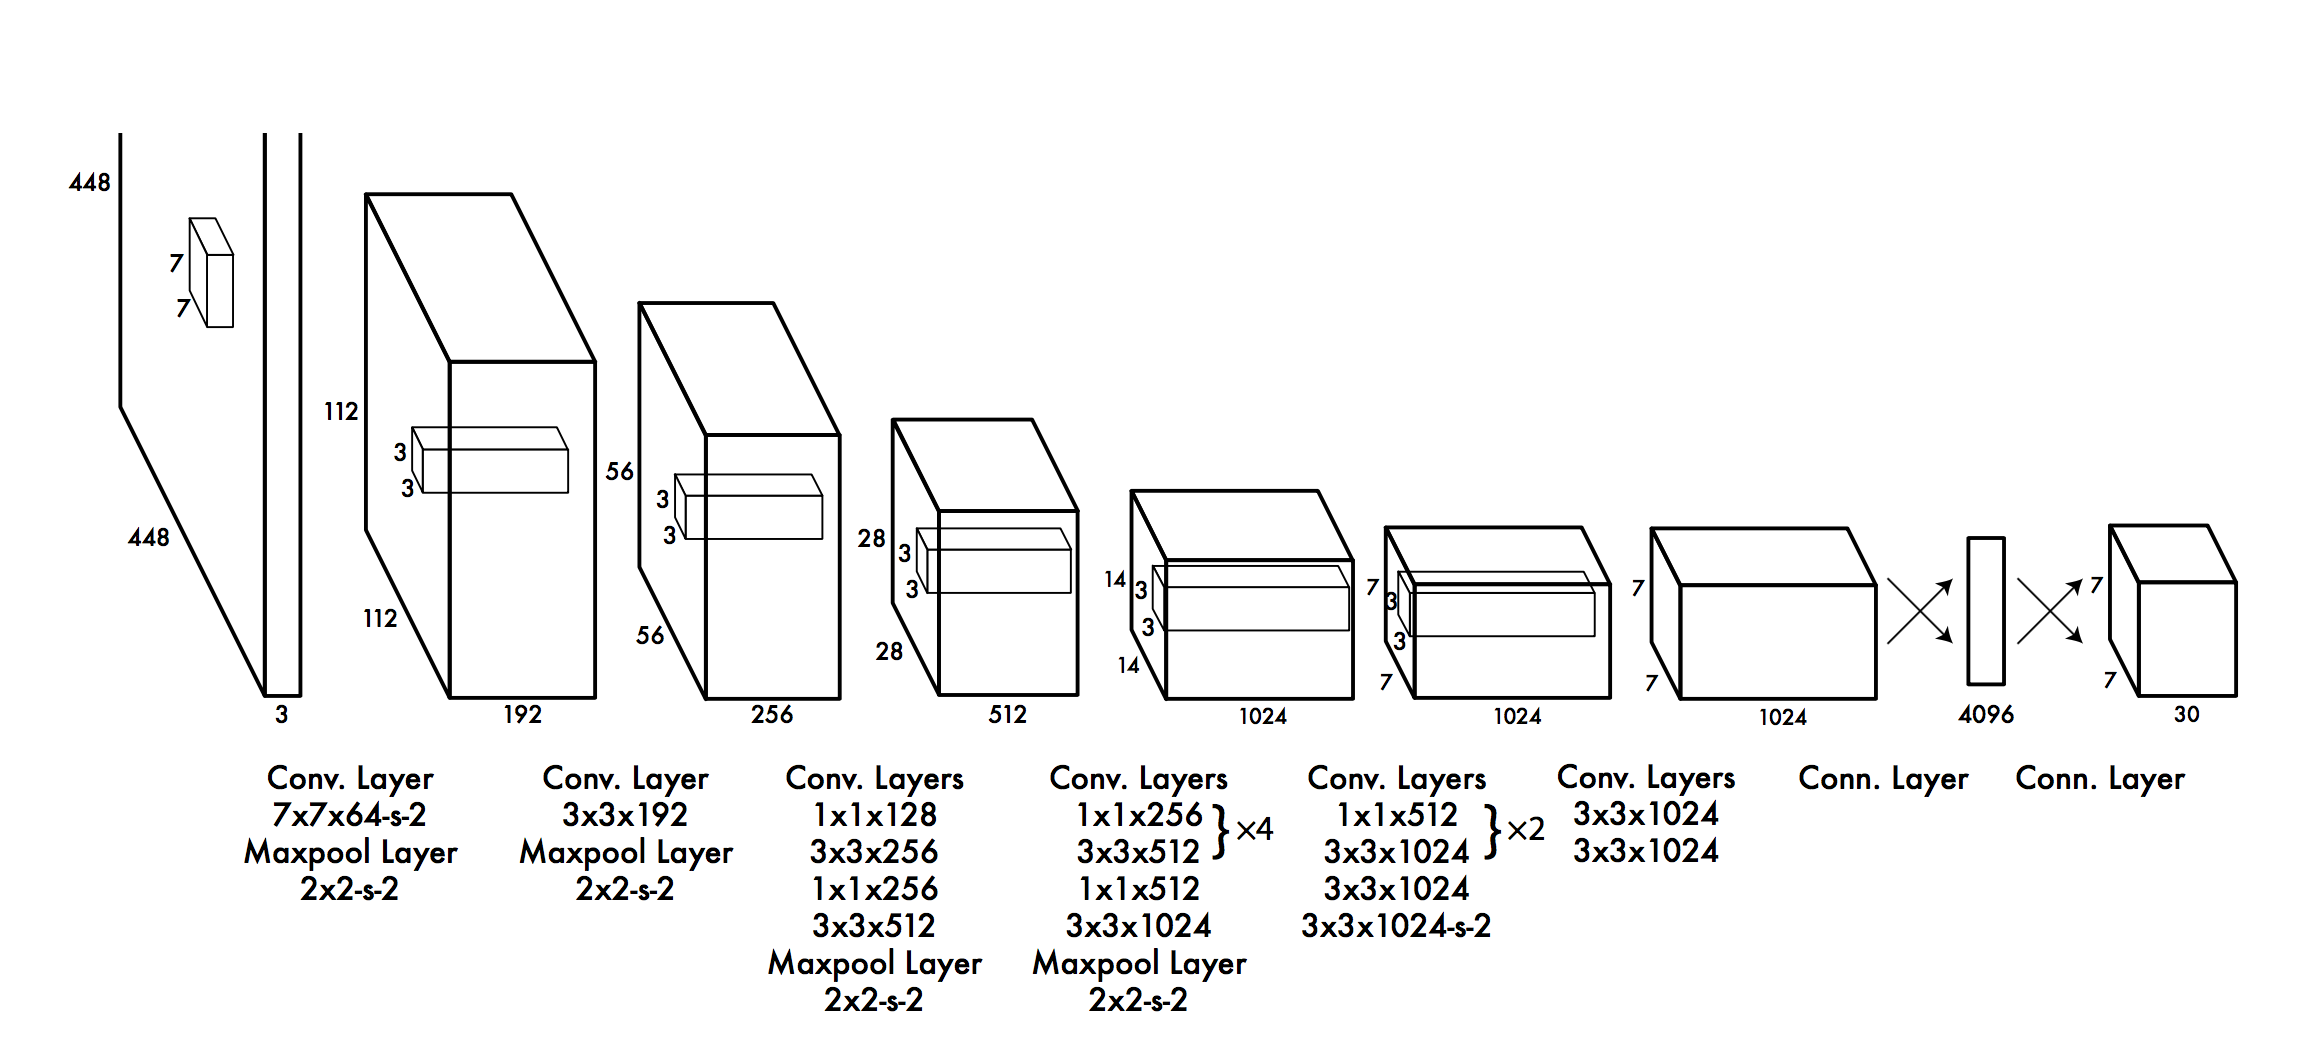
\includegraphics[width=1.0\linewidth]{img/yolo_network.png}
    \caption{Yolo Network Architecture}
\end{figure}%


\subsection{Faster R-CNN}
Faster R-CNN is an elegant and effective solution for object detection. 
It is an end-to-end object detection framework using a Region Proposal Network (RPN) and an Object Detection Network. Previous methods such as SPPnet and Fast R-CNN, reply on proposal algorithms to hypothesize object locations, which becomes a bottleneck in order to reducing the running time. In Faster R-CNN, we don't need to pre-generated several region proposals using some inexpensive features and economical inference schemes such as Selective Search. Instead, it has a RPN on top of the convolutional features, which can be used for generating detection proposals and be trained end-to-end. 

A Region Proposal Network (RPN) takes an image (of any size) as input and outputs a set of rectangular object proposals, each with an objectness score. Such process is modeled by a fully convolution network \cite{long2015fully}. The region proposals are generated by 
the box-regression layer and box-classification layer using the features from a small network sliding over the convolutional feature map output. 

After generating a set of object proposals using RPNs, Fast R-CNN can be using to make detection. And since RPN and Fast R-CNN all rely on some convolutional neural networks, Faster R-CNN make them share some convolutional layers to make it converge quickly.
